\title{Second Update on Polygon Detection Algorithm}
\author{
        Andrew Ho \\
        Aerospace Robotics and Control Laboratory \\
        California Institute of Technology \\
}

\documentclass[12pt]{article}
\usepackage{graphicx}
\usepackage{float}
\graphicspath{ {./images/} }

\begin{document}
\maketitle

\section{Introduction}

\noindent The goal of the image processing stage is to extract line segments which correspond
to true edges or at least to edges available in the spacecraft model. In combination with Polygon tracking, the project aims to find a robust method of mapping polygons.

\section{Pipeline}

We use the following pipeline to detect line segments within an image, in order to detect larger polygons:

\begin{enumerate}
\item Low Pass Filtering
\item Thresholding
\item Edge Detection
\item Corner Detection
\item Convex Hull 
\item Further Corner Filtering
\item Polygon Tracking
\end{enumerate}

\noindent Low Pass Filtering: This step reduces contrast within image, effectively blurring out less important edges. This allows for higher accuracy when we apply edge detection algorithms. \newline

\noindent Thresholding:  This step strips the image down to strong features, removing external noise in an image. \newline

\noindent Edge Detection: This step implements two different edge detection algorithms. First, Probabilistic Hough Line Transform is applied, extracting an array of important segments. Then the Line Segment Detector algorithm outlined in:\newline
 
 \indent Rafael Grompone von Gioi, J�r�mie Jakubowicz, Jean-Michel Morel, and Gregory Randall. Lsd: a line segment detector. 2012. \newline
 
\noindent is used to thin out the edges detected from Hough Line Transform. \newline

\noindent Corner Detection: This step implements the Shi-Tomasi method of detecting corners. We apply this algorithm to the stripped image from Edge Detection. We set the max number of corners to 8, casting a wide net in case the true corners to detect are not the strongest corners in the image. \newline

\noindent Convex Hull: This step takes the corners detected in the Corner Detection step and finds the convex hull of outer most points, guaranteeing that we preserve true corners. \newline

\noindent Further Corner Filtering: This step takes the points of the Convex Hull and removes collinear points, leaving only true corners. From these true corners we draw edges to outline the polygon. \newline

\section{Example Process}

\noindent Consider the following image:\newline

\begin{figure}[H]
\caption{Original Source Image}
\centering
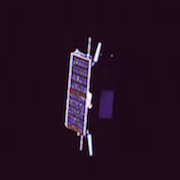
\includegraphics{source}
\end{figure}

\noindent To the human eye, the white rectangle is quite evident. However, there are certain issues for a computer. The bottom length of the rectangle is missing and the antennae of the satellites may prove to turn up as false corners.

\noindent We would like to receive a polygon from the image, as shown in the following image: \newline

\begin{figure}[H]
\caption{Desired Output}
\centering
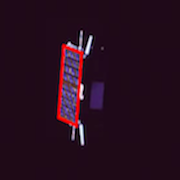
\includegraphics{desired_result}
\end{figure}

\noindent First, we apply thresholding: \newline

\begin{figure}[H]
\caption{Thresholding}
\centering
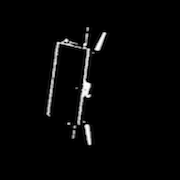
\includegraphics{threshold}
\end{figure}

\noindent Second, we apply Probabilistic Hough Line Transform: \newline

\begin{figure}[H]
\caption{Probabilistic Hough Line Transform}
\centering
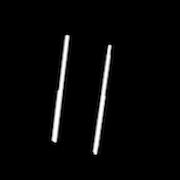
\includegraphics{hough}
\end{figure} 

\noindent To this image, we apply the Line Segment Detector algorithm from Grompone, Jakubowicz, Morel, and Randall: \newline

\begin{figure}[H]
\caption{Line Segment Detector}
\centering
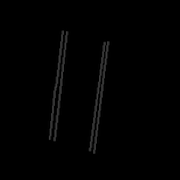
\includegraphics{LSD}
\end{figure}

\noindent Next, we use the Shi-Tomasi algorithm to detect important corners: \newline

\begin{figure}[H]
\caption{Shi-Tomasi Corner Detection}
\centering
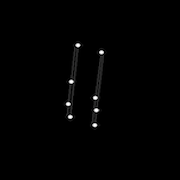
\includegraphics{corner_detection}
\end{figure}

\noindent Notice we have over-detected corners. This is to ensure we capture true corners. Next, we find the convex hull: \newline

\begin{figure}[H]
\caption{Convex Hull}
\centering
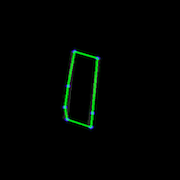
\includegraphics{convex_hull}
\end{figure}

\noindent From the convex hull, we remove collinear lines, leaving us with a simple polygon: \newline

\begin{figure}[H]
\caption{Filtered Convex Hull}
\centering
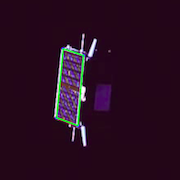
\includegraphics{progression_final}
\end{figure}

\noindent Compared to our target polygon, the algorithm does a tremendous job of finding the correct polygon: \newline

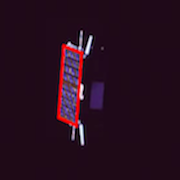
\includegraphics{desired_result}    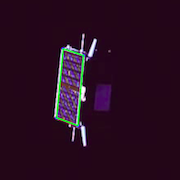
\includegraphics{progression_final} \newline

\noindent Below are additional examples compared side by side: \newline

\noindent Example 1 \newline 

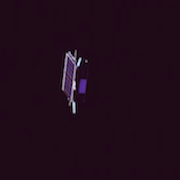
\includegraphics{source2}    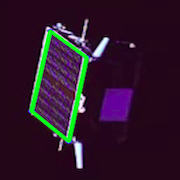
\includegraphics{result2} \newline



\noindent Example 2 \newline

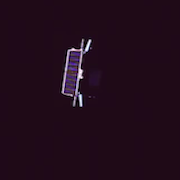
\includegraphics{source3}    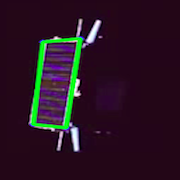
\includegraphics{result3} \newline


\section {Next Steps and Challenges}
	There are certain cases in which the antennae provides too strong of a corner. Consider the following image:
	
\begin{figure}[H]
\caption{Failure Example}
\centering
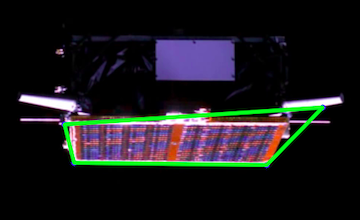
\includegraphics{failure_case}
\end{figure}

From the Harris Corner Detection step output, it's clear to see that there is an extra corner detected that skews the results

\begin{figure}[H]
\caption{Harris Corner Detection Failure}
\centering
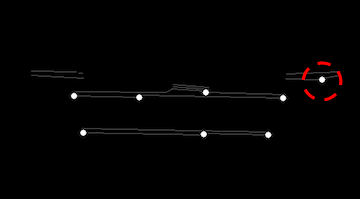
\includegraphics{harris_failure}
\end{figure}
	
	To amend this issue, we can instead implement a Traveling Salesman algorithm to find include every point in the outer layer, and detect whether or not corners detected are legitimate by comparing whether pixels between the points are black or white. If there are not enough pixels between two corners that are white, then that corner must not exist.

\bibliographystyle{abbrv}
\bibliography{main} 

\end{document}